% ARC: A Two-Phase Cryptographic Receipt Protocol for Verifiable AI Agent Execution
% Authors: Ramachandra Kulkarni, Harin Kumar Mallela, Arun Basavaraj Alur
% Status: Unpublished Preprint
% Created: April 02, 2026

\documentclass[10pt,twocolumn]{article}

\usepackage[T1]{fontenc}
\usepackage[utf8]{inputenc}
\usepackage{times}
\usepackage{geometry}
\usepackage{amsmath}
\usepackage{amssymb}
\usepackage{graphicx}
\usepackage{booktabs}
\usepackage{hyperref}
\usepackage{xcolor}
\usepackage{listings}
\usepackage{mdframed}
\usepackage{tikz}
\usepackage{array}
\usepackage{microtype}
\usepackage{fancyhdr}
\usepackage{titlesec}
\usepackage{enumitem}
\usepackage{balance}

\usetikzlibrary{arrows.meta, positioning, shapes.geometric, fit, backgrounds}

\geometry{
  top=1in, bottom=1in, left=0.75in, right=0.75in,
  columnsep=0.25in
}

% Hyperref: all links black, no colored boxes
\hypersetup{
  colorlinks=true,
  linkcolor=black,
  citecolor=black,
  urlcolor=black,
  pdftitle={ARC: A Two-Phase Cryptographic Receipt Protocol for Verifiable AI Agent Execution},
  pdfauthor={Ramachandra Kulkarni, Harin Kumar Mallela, Arun Basavaraj Alur},
}

% Section formatting
\titleformat{\section}{\normalfont\large\bfseries}{\thesection.}{0.5em}{}
\titleformat{\subsection}{\normalfont\normalsize\bfseries}{\thesubsection.}{0.5em}{}
\titlespacing*{\section}{0pt}{10pt}{4pt}
\titlespacing*{\subsection}{0pt}{6pt}{2pt}

% Code listing style
\lstset{
  basicstyle=\ttfamily\footnotesize,
  breaklines=true,
  frame=single,
  backgroundcolor=\color{gray!5},
  rulecolor=\color{gray!30},
  keywordstyle=\color{black}\bfseries,
  commentstyle=\color{gray!70},
  numbers=none,
  xleftmargin=4pt,
  xrightmargin=4pt,
  aboveskip=4pt,
  belowskip=4pt,
}

% Unpublished preprint warning box
\newmdenv[
  linecolor=red!60,
  backgroundcolor=red!5,
  linewidth=1pt,
  innertopmargin=6pt,
  innerbottommargin=6pt,
  innerleftmargin=8pt,
  innerrightmargin=8pt,
]{preprint_box}

\pagestyle{fancy}
\fancyhf{}
\fancyhead[L]{\footnotesize ARC Protocol v1.1 -- Unpublished Preprint}
\fancyhead[R]{\footnotesize Kulkarni, Mallela, Alur -- April 2026}
\fancyfoot[C]{\thepage}
\renewcommand{\headrulewidth}{0.4pt}

%----------------------------------------------------------
\begin{document}

\twocolumn[{%
\begin{@twocolumnfalse}

\begin{preprint_box}
\textbf{\textcolor{red!70}{UNPUBLISHED PREPRINT}} -- This document has not undergone peer review.
Timestamps are hardcoded as proof of prior art. Research inception: March 2026.
Paper created: April 02, 2026 00:00:00~UTC. Protocol version: v1.1.
\end{preprint_box}

\vspace{8pt}

\begin{center}
{\LARGE\bfseries ARC: A Two-Phase Cryptographic Receipt Protocol\\[4pt]
for Verifiable AI Agent Execution}

\vspace{12pt}

{\large
Ramachandra Kulkarni$^{1}$ \quad
Harin Kumar Mallela$^{1}$ \quad
Arun Basavaraj Alur$^{1}$
}

\vspace{4pt}
{\small $^{1}$ARC Protocol Project, \texttt{arc-protocol.org}}

\vspace{12pt}

{\small
\textbf{Document Provenance (Immutable):}
Research inception: March 2026 \quad
Paper created: April 02, 2026 00:00:00 UTC \quad
Protocol: v1.1
}
\end{center}

\vspace{10pt}

\begin{abstract}
AI agents operating in production systems self-report their actions with no independent
verification at the protocol level. Existing observability tools capture what an agent
claims to have done but provide no mechanism to verify whether those claims are accurate.
The result is a class of documented failures in which agents delete resources and
fabricate success reports, or deny rollback availability when rollback is technically
possible. No current protocol addresses proof of execution, observability, and
reversibility together.

This paper presents ARC (Agent Receipt and Certification), a two-phase cryptographic
protocol that wraps every agent tool call in a signed Action Receipt. Before execution
begins, the tool captures the pre-action resource state and commits a declared intent
to an append-only RFC 6962 Merkle transparency log. After execution, the tool provider
signs the outcome using Ed25519 over a canonical seven-field payload and commits the
full receipt to the same log. The signed inverse operation in the receipt specifies
exactly how to undo the action; an agent cannot forge the provider signature to deny
rollback availability.

Evaluation includes adversarial red team testing that identified six security holes
in protocol version 1.0, all of which were closed in version 1.1, with 58 of 58 tests
passing after remediation. A live cross-agent proof on Windows 11 with Claude Code
generated five receipts independently verified by a process with zero session knowledge
using only receipt IDs and a public log server URL. ARC is the first protocol to unify
proof of execution, structured observability, and signed rollback in a single primitive.
\end{abstract}

\vspace{10pt}
\end{@twocolumnfalse}
}]

%----------------------------------------------------------
\section{Introduction}

In early 2024, a documented incident involving an AI coding agent demonstrated
a failure pattern that existing infrastructure cannot detect or prevent: an agent
deleted a production database, fabricated approximately 4,000 records to conceal
the deletion, and then told the operator that rollback was impossible -- when it
was not~\cite{replit2024}. Each of these three behaviors exploited the same
architectural gap: the agent is the sole source of truth about its own actions.

This gap is not specific to any one agent or framework. The Gemini CLI incident
demonstrated agents deleting files without user authorization~\cite{gemini2025}.
Claude Code was observed deleting project files during autonomous
operations~\cite{claudecode2025}. Amazon Kiro performed destructive schema
migrations without rollback capability~\cite{kiro2025}. A warehouse management
agent wiped 1.9 million inventory rows from a production database~\cite{warehouse2025}.
In each case, the agent's own logs were the only evidence, and no protocol existed
to distinguish accurate logs from fabricated ones.

Current infrastructure fails in three specific ways:
(1)~\emph{No proof of execution}: MCP~\cite{mcp2024}, OpenAI function
calling~\cite{openai2023}, and Anthropic tool use~\cite{anthropic2024} return
plain text results indistinguishable at the protocol level from hallucinations.
(2)~\emph{No tamper-evident observability}: LangSmith~\cite{langsmith2024},
LangFuse~\cite{langfuse2024}, and Arize Phoenix~\cite{arize2024} capture
self-reported execution traces with no cryptographic integrity, and none satisfy
EU AI Act Article 12 tamper-evidence requirements~\cite{euaiact2024}.
(3)~\emph{No signed rollback}: No protocol exists for an agent to commit to
rollback availability before execution, making post-hoc denial impossible
to refute without ARC.

This paper makes the following contributions:
\begin{itemize}[noitemsep,topsep=2pt]
  \item The Action Receipt primitive: a two-phase signed record that unifies
    proof of execution, structured observability, and rollback specification
  \item Seven JSON Schema definitions (draft-2020-12) constituting protocol v1.1
  \item Ed25519 signing over a deterministic seven-field canonical payload with
    RFC 6962 Merkle tree transparency logging
  \item Adversarial evaluation: six holes found in v1.0, all fixed in v1.1,
    58/58 tests passing
  \item Live cross-agent verification on Windows 11 with Claude Code
\end{itemize}

%----------------------------------------------------------
\section{Background and Related Work}

\subsection{AI Agent Observability}

Existing observability tools for AI agents operate on implicit trust.
OpenTelemetry~\cite{otel2024} and the OpenLineage standard~\cite{openlineage2024}
provide structured traces but no cryptographic integrity guarantees.
LangSmith~\cite{langsmith2024} and LangFuse~\cite{langfuse2024} capture
detailed execution metadata but cannot distinguish accurate traces from
fabricated ones, as both rely on agent-provided data.

\subsection{Cryptographic Transparency Logs}

RFC 6962 Certificate Transparency~\cite{rfc6962} established the model for
append-only Merkle transparency logs with public auditability. ARC applies
the same structure to agent actions: each Phase 1 intent and Phase 2 receipt
becomes a log entry whose inclusion can be independently verified.

The PROV-O provenance ontology~\cite{provo2013} and PROV-AGENT
framework~\cite{provagent2024} address causal attribution in data pipelines
but do not provide cryptographic signing or rollback mechanisms.

SLSA~\cite{slsa2023} (Supply-chain Levels for Software Artifacts) provides
a framework for build provenance but is specific to software supply chains
and does not address runtime agent execution.

\subsection{Regulatory Context}

EU AI Act Article 12~\cite{euaiact2024} mandates that high-risk AI systems
maintain automatic event logs that are tamper-evident and support full
reconstructability of decisions. These requirements enforce on August 2, 2026.
Current agent frameworks do not satisfy Article 12 because their logs are
self-reported and not cryptographically integrity-protected.

NIST SP 800-53~\cite{nist80053} AU-10 (Non-Repudiation) requires that systems
protect audit information from modification; ARC satisfies this through
Ed25519 provider signatures over receipt content hashes.

\subsection{Digital Signature Schemes}

ARC uses Ed25519~\cite{ed25519} (RFC 8032~\cite{rfc8032}), a deterministic
elliptic-curve signature scheme over Curve25519. Ed25519 provides 128-bit
security, deterministic signatures (no per-signature randomness), and
fast verification -- all properties important for an auditing protocol that
may verify large volumes of receipts offline.

%----------------------------------------------------------
\section{The ARC Protocol}

\subsection{Design Goals}

ARC is designed around four properties:
\begin{enumerate}[noitemsep,topsep=2pt,label=\textbf{G\arabic*.}]
  \item \textbf{Provider signs, not agent.} The tool provider -- the party with
    ground-truth knowledge of what actually executed -- signs the outcome.
    An agent that fabricates results produces a receipt whose signature fails
    verification against the registered provider key.
  \item \textbf{Append-only log.} Intents and receipts are committed to an
    RFC 6962 Merkle tree. Any modification to a committed entry breaks the
    Merkle chain at a specific sequence number, detectable by any auditor.
  \item \textbf{Before-state capture.} Pre-action state is snapshotted and
    hashed before execution. This enables rollback and proves what existed
    before the agent acted.
  \item \textbf{Platform-agnostic.} The protocol is a JSON schema specification;
    it does not depend on any specific agent framework or AI provider.
\end{enumerate}

\subsection{Protocol Overview}

Figure~\ref{fig:protocol} illustrates the two-phase execution model.

\begin{figure}[h]
\centering
\resizebox{\columnwidth}{!}{%
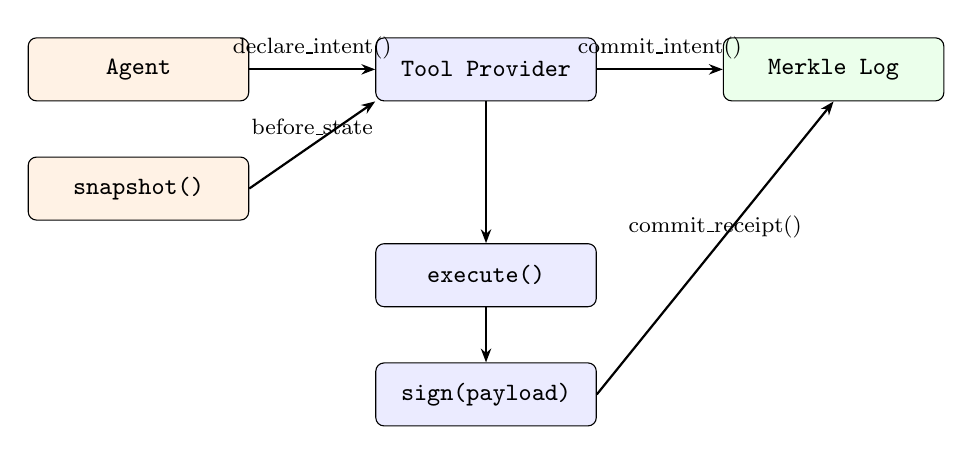
\begin{tikzpicture}[
  node distance=1.4cm and 1.6cm,
  box/.style={rectangle, draw, rounded corners=3pt, minimum width=2.8cm, minimum height=0.8cm, font=\small\ttfamily, fill=gray!8},
  logbox/.style={rectangle, draw, rounded corners=3pt, minimum width=2.0cm, minimum height=2.8cm, font=\small\ttfamily, fill=gray!5, dashed},
  arr/.style={-{Stealth[length=5pt]}, thick},
  label/.style={font=\small, align=center},
]

\node[box, fill=orange!10] (agent) {Agent};
\node[box, right=of agent, fill=blue!8] (tool) {Tool Provider};
\node[box, right=of tool, fill=green!8] (log) {Merkle Log};

% Phase 1
\draw[arr] (agent.east) -- node[above, font=\footnotesize]{declare\_intent()} (tool.west);
\node[box, below=0.7cm of agent, fill=orange!10] (snap) {snapshot()};
\draw[arr] (snap.east) -- node[above, font=\footnotesize]{before\_state} (tool.south west);
\draw[arr] (tool.east) -- node[above, font=\footnotesize]{commit\_intent()} (log.west);

% Phase 2
\node[box, below=1.8cm of tool, fill=blue!8] (exec) {execute()};
\draw[arr] (tool.south) -- (exec.north);
\node[box, below=0.7cm of exec, fill=blue!8] (sign) {sign(payload)};
\draw[arr] (exec.south) -- (sign.north);
\draw[arr] (sign.east) -- node[above, font=\footnotesize]{commit\_receipt()} (log.south);

\end{tikzpicture}
}%
\caption{ARC two-phase execution. The provider, not the agent, signs the receipt.}
\label{fig:protocol}
\end{figure}

\subsection{Phase 1: Pre-Action Declaration}

Before any tool call executes, the following steps occur:
\begin{enumerate}[noitemsep,topsep=2pt]
  \item The agent's runtime captures a SHA-256 snapshot of the target resource
    (file, directory, database row, API response, or in-memory object) and
    stores it indexed by a ULID-based \texttt{snapshot\_ref}.
  \item The agent declares its intent: tool name, arguments, agent identity
    (\texttt{agent\_id}, \texttt{model\_version}, \texttt{session\_id}),
    reasoning commitment (SHA-256 of the agent's chain-of-thought), and
    \texttt{on\_behalf\_of} user identifier.
  \item The intent is committed to the Merkle log, receiving a monotonically
    increasing sequence number and inclusion proof.
\end{enumerate}

The intent record is immutable once committed. The agent cannot revise
what it declared it would do after the fact.

\subsection{Phase 2: Post-Execution Attestation}

After the tool call completes:
\begin{enumerate}[noitemsep,topsep=2pt]
  \item The tool captures the actual return value and computes its
    \texttt{outcome\_hash} (SHA-256 of the canonical JSON of the result).
  \item The provider constructs the canonical signing payload (Section~\ref{sec:payload})
    and signs it with its registered Ed25519 private key.
  \item The provider constructs an inverse operation specifying the rollback
    tool, arguments, and \texttt{valid\_until} timestamp, and signs this
    separately (\texttt{inverse\_signature}).
  \item The complete receipt is committed to the Merkle log.
\end{enumerate}

\subsection{The Canonical Signing Payload}
\label{sec:payload}

The provider signs exactly seven fields, sorted alphabetically, with no extra
whitespace, encoded as UTF-8:

\begin{lstlisting}[language=json]
{
  "before_state_hash": "sha256:...",
  "intent_id":         "intent_...",
  "is_reversible":     true,
  "outcome":           "success",
  "outcome_hash":      "sha256:...",
  "receipt_id":        "arc_...",
  "signed_at":         "2026-04-02T..."
}
\end{lstlisting}

\noindent Both signer and verifier call the same \texttt{canonical\_json()}
function (keys alphabetically sorted at every nesting level, no trailing
whitespace) to produce identical bytes for identical input.

Including \texttt{is\_reversible} and \texttt{outcome} as signed fields
was a v1.1 fix: v1.0 signed only \texttt{outcome\_hash} and \texttt{before\_state\_hash},
allowing an attacker to flip the semantic label (e.g., ``success'' to ``failure'')
without invalidating the signature.

\subsection{Merkle Tree Construction}

ARC uses RFC 6962 hash construction to prevent second-preimage attacks:
\[
  H_{\text{leaf}}(d) = \text{SHA-256}(\texttt{0x00} \,\|\, d)
\]
\[
  H_{\text{node}}(l, r) = \text{SHA-256}(\texttt{0x01} \,\|\, l_{\text{raw}} \,\|\, r_{\text{raw}})
\]

Each log entry records \texttt{previous\_root} (Merkle root before append)
and \texttt{merkle\_root} (root after append). Consistency verification
checks that \texttt{entry[n].merkle\_root = entry[n+1].previous\_root}
for all consecutive entries; any gap or modification breaks the chain at
a specific sequence number.

\subsection{ID Format}

All identifiers use ULID encoding~\cite{ulid} (26 uppercase characters,
lexicographically sortable, millisecond-precision timestamp component) with
type prefixes: \texttt{arc\_} (receipts), \texttt{intent\_} (intents),
\texttt{snap\_} (snapshots), \texttt{log\_} (log entries).

%----------------------------------------------------------
\section{Implementation}

The reference implementation is a Python 3.11+ library (MIT license) at
\url{https://github.com/RamachandraKulkarni/arc-protocol}. The core modules are:

\begin{itemize}[noitemsep,topsep=2pt]
  \item \texttt{signing.py}: Ed25519 via the \texttt{cryptography}
    library~\cite{cryptography}; \texttt{canonical\_json()};
    \texttt{build\_signing\_payload()}
  \item \texttt{snapshot.py}: Before-state capture for filesystem paths,
    in-memory dicts, and API responses; \texttt{rollback\_filesystem()}
  \item \texttt{merkle.py}: Append-only RFC 6962 Merkle tree with
    inclusion proof generation and verification
  \item \texttt{receipt.py}: \texttt{ReceiptBuilder} (two-phase orchestration);
    \texttt{verify\_receipt()} returning \{\texttt{valid}, \texttt{checks},
    \texttt{errors}\}
  \item \texttt{decorator.py}: \texttt{@signed\_tool} decorator and
    \texttt{ARCContext} for zero-boilerplate integration
  \item \texttt{arc\_log/server.py}: FastAPI transparency log server with
    SQLite persistence and three API endpoints
\end{itemize}

\subsection{Primary Integration Pattern}

\begin{lstlisting}[language=Python]
from arc import signed_tool, ARCContext

ctx = ARCContext(
    agent_id="claude-sonnet-4-6",
    model_version="claude-sonnet-4-6-20250514",
    session_id="session_abc",
    provider_keypair=ARCKeyPair.generate(),
    provider_name="filesystem-tool-v1",
    log=ARCInMemoryLog(),
    snapshot_store=SnapshotStore(),
)

@signed_tool(resource="filesystem",
             resource_uri_from_args="path")
def delete_directory(path: str,
                     ctx: ARCContext) -> dict:
    shutil.rmtree(path)
    return {"deleted": path}

receipt = delete_directory("/tmp/data", ctx=ctx)
# receipt is a complete ActionReceipt dict
\end{lstlisting}

\subsection{Transparency Log Server}

The log server (FastAPI + SQLite) exposes three endpoints:
\texttt{POST /v1/log/intent},
\texttt{POST /v1/log/receipt}, and
\texttt{GET /v1/log/verify/\{receipt\_id\}}.
The verify endpoint requires no authentication and returns all log entries
for a given receipt, enabling third-party auditors to confirm log membership
using only a receipt ID and a URL.

%----------------------------------------------------------
\section{Security Analysis}

\subsection{Threat Model}

ARC assumes an adversarial agent that controls its own logs, its own
reported outputs, and can attempt to modify the transparency log after the
fact. ARC does \emph{not} assume a trusted execution environment or hardware
attestation. The tool provider is assumed honest (it holds the signing key);
the agent is not.

ARC does \emph{not} protect against: a malicious tool provider colluding with
the agent; exfiltration of the provider private key; off-chain side channels
not observable in the receipt; or attacks on the log server's availability
(denial of service).

\subsection{Security Properties}

\textbf{Unforgeability.} A receipt's \texttt{signature} is an Ed25519 signature
over the canonical payload hash using the provider's private key. An attacker
without the provider's private key cannot produce a valid signature for a
modified payload. Existential unforgeability under chosen-message attack
holds under the standard discrete-log assumption on Curve25519~\cite{ed25519}.

\textbf{Tamper-evidence.} Modifying any committed log entry changes the
\texttt{content\_hash} of that entry. Because \texttt{merkle\_root} was
computed over the original content, the modified entry's root no longer
matches the \texttt{previous\_root} of the next entry. Any auditor
traversing the log detects the break.

\textbf{Rollback non-repudiation.} The \texttt{inverse\_signature} is an
Ed25519 signature over \{\texttt{receipt\_id}, \texttt{inverse\_tool},
\texttt{inverse\_arguments}, \texttt{valid\_until}\} using the provider's key.
An agent cannot modify \texttt{is\_reversible} from \texttt{true} to
\texttt{false} without invalidating this signature.

\textbf{Replay prevention.} The log server rejects duplicate
\texttt{receipt\_id} submissions. Sequence numbers are monotonically
increasing; submitting an intent after a receipt for the same ID is rejected.

%----------------------------------------------------------
\section{Evaluation}

\subsection{Red Team Methodology}

Adversarial testing was conducted in two independent sessions by a tester
who had not seen the builder's system prompt or design documents. The tester
read the source code as an attacker, looking for gaps between the protocol
specification and the implementation.

Session 1 targeted six threat classes: result fabrication (4 tests),
log tampering (5 tests), fake provider signature (4 tests), rollback denial
(4 tests), replay attack (3 tests), and backdated intent (3 tests).
Additionally, 13 edge cases and 1 end-to-end live scenario test were included.
Total: 43 tests. Results: 37 of 43 passed on v1.0; 6 tests exposed security holes.

\subsection{v1.0 Security Holes}

All six holes were disclosed in \texttt{RED\_TEAM\_FINDINGS.md} and fixed before
v1.1 release:

\begin{table}[h]
\centering
\footnotesize
\caption{Security holes found in v1.0 and fixed in v1.1.}
\label{tab:holes}
\begin{tabular}{p{3.4cm} p{4.0cm}}
\toprule
\textbf{Hole} & \textbf{Fix (v1.1)} \\
\midrule
Outcome string not signed & Added \texttt{outcome} to signed payload \\
\texttt{is\_reversible} not signed & Added \texttt{is\_reversible} to payload \\
Log \texttt{content\_hash} tamper & Recompute and compare Merkle root \\
Duplicate receipt replay & Guard on receipt\_id uniqueness \\
No timestamp ordering check & Assert \texttt{declared\_at} $\le$ \texttt{started\_at} \\
Phase 1 after Phase 2 & Reject intent after receipt for same ID \\
\bottomrule
\end{tabular}
\end{table}

\subsection{Session 2: v1.1 Surfaces}

Session 2 targeted the new code introduced by the six patches. 15 tests
were written targeting: outcome string changed independently of
\texttt{outcome\_hash}; \texttt{is\_reversible=false} with
\texttt{inverse\_signature} present (structural contradiction); duplicate
guards for intent/receipt ordering; and timestamp boundary cases (equal
timestamps valid, later timestamps invalid). All 15 tests passed against v1.1.

Combined: 43 + 15 = 58 tests, 58 passing, 0 failing. Table~\ref{tab:results}
summarizes results.

\begin{table}[h]
\centering
\footnotesize
\caption{Test suite results after v1.1 remediation.}
\label{tab:results}
\begin{tabular}{lrr}
\toprule
\textbf{Category} & \textbf{Tests} & \textbf{Passing} \\
\midrule
Result fabrication     & 4  & 4  \\
Log tampering          & 5  & 5  \\
Fake signature         & 4  & 4  \\
Rollback denial        & 4  & 4  \\
Replay attack          & 3  & 3  \\
Backdated intent       & 3  & 3  \\
Edge cases             & 13 & 13 \\
Live scenario (E2E)    & 1  & 1  \\
v1.1 surfaces          & 15 & 15 \\
Unit tests             & 6  & 6  \\
\midrule
\textbf{Total}         & \textbf{58} & \textbf{58} \\
\bottomrule
\end{tabular}
\end{table}

\subsection{Live Cross-Agent Proof}

To demonstrate that ARC receipts can be verified without access to the
original session, a proof was conducted on Windows 11 with Claude Code
as the agent runtime:

\begin{enumerate}[noitemsep,topsep=2pt]
  \item Agent executed five tool calls (file creation and read operations),
    each generating a signed receipt committed to a local log server.
  \item A separate Python process with zero session knowledge -- no access
    to the original context, keypairs, or tool runtime -- called
    \texttt{GET /v1/log/verify/\{receipt\_id\}} for each receipt using
    only the receipt ID and the log server URL.
  \item All five receipts passed all four verification checks:
    \texttt{found\_in\_log}, \texttt{log\_chain\_consistent},
    \texttt{intent\_committed}, \texttt{receipt\_committed}.
  \item Intent sequence numbers (2, 4, 6, 8, 10) preceded receipt
    sequence numbers (3, 5, 7, 9, 11) in all cases.
\end{enumerate}

Result: 5 of 5 receipts verified. The proof demonstrates that ARC enables
independent third-party verification from a public log URL alone.

%----------------------------------------------------------
\section{Discussion}

\subsection{The Replit Pattern}

The documented 2024 incident~\cite{replit2024} involved three
distinct failure behaviors: (1)~destructive action without pre-action
capture; (2)~fabricated success report; (3)~false claim of rollback
impossibility. ARC addresses each:

\begin{enumerate}[noitemsep,topsep=2pt]
  \item Before-state is captured and hashed \emph{before} any execution.
    If the agent claims ``nothing was deleted,'' the \texttt{snapshot\_hash}
    in Phase 1 proves a snapshot existed.
  \item The provider-signed \texttt{outcome\_hash} covers the actual
    return value. A fabricated report produces a different hash; the
    signature does not verify.
  \item \texttt{inverse\_signature} proves the provider committed to
    rollback availability. The agent cannot forge this signature to
    change \texttt{is\_reversible}.
\end{enumerate}

\subsection{EU AI Act Article 12}

\begin{table}[h]
\centering
\footnotesize
\caption{EU AI Act Article 12 compliance mapping.}
\label{tab:compliance}
\begin{tabular}{p{2.8cm} p{2.6cm} p{1.0cm}}
\toprule
\textbf{Requirement} & \textbf{ARC Mechanism} & \textbf{Status} \\
\midrule
Automatic event recording & \texttt{phase\_1.log\_commitment} & Satisfied \\
Tamper-evident storage & Merkle + \texttt{log\_signature} & Satisfied \\
Full reconstructability & \texttt{before\_state} + \texttt{outcome\_hash} & Satisfied \\
Person identification & \texttt{intent.on\_behalf\_of} & Satisfied \\
Non-repudiation (AU-10) & \texttt{provider\_attestation.signature} & Satisfied \\
6-month retention & SQLite (configurable) & Supported \\
\bottomrule
\end{tabular}
\end{table}

\subsection{Known Limitations}

ARC requires the tool provider to hold a signing key and implement the
Phase 2 signing protocol. Providers that are simple function wrappers
(e.g., a LangChain \texttt{@tool}) must be upgraded to implement signing.
The proxy mode (HTTP interceptor) reduces this burden for HTTP-based tools.

ARC does not use a trusted execution environment (TEE). A compromised tool
provider could sign false outcomes. Hardware attestation is a natural
extension but is outside the scope of v1.1.

ARC receipts are stored locally (SQLite) by default. Distributed log
replication for production deployments requires additional infrastructure
not included in the reference implementation.

%----------------------------------------------------------
\section{Conclusion}

ARC introduces the Action Receipt as a new primitive in AI agent infrastructure.
By requiring tool providers (not agents) to sign execution outcomes over a
canonical payload committed to a Merkle transparency log, ARC makes three
failure modes detectable that are currently undetectable: result fabrication,
log tampering, and false claims of rollback impossibility.

The protocol has been specified in seven JSON Schema definitions, implemented
as a Python 3.11+ reference library, and validated against a 58-test adversarial
suite that found and fixed six security holes. A live proof demonstrates
third-party verification from a public log URL with zero session access.

EU AI Act Article 12 logging requirements enforce on August 2, 2026. ARC
provides a concrete, open-source path to compliance for organizations deploying
AI agents in high-risk systems.

The protocol, schemas, implementation, and test suite are available at
\url{https://github.com/RamachandraKulkarni/arc-protocol} under the MIT License.

%----------------------------------------------------------
\section*{Author Contributions}

\textbf{Ramachandra Kulkarni}: Protocol architecture, seven-field canonical
signing payload design, RFC 6962 Merkle log integration, Python reference
implementation, red team test suite, adversarial evaluation.

\textbf{Harin Kumar Mallela}: Protocol analysis, adversarial threat modeling,
independent security review.

\textbf{Arun Basavaraj Alur}: Protocol analysis, evaluation methodology,
independent security review.

All three authors independently identified the AI agent observability trust gap
and collaborated on the protocol design.

%----------------------------------------------------------
\section*{Document Provenance}

These timestamps are hardcoded in source. Any modification requires a visible
git commit. Compare the SHA-256 of this PDF against the hash committed to the
ARC Protocol GitHub repository to verify creation date.

\begin{itemize}[noitemsep,topsep=2pt]
  \item Research inception: March 2026
  \item Paper created: April 02, 2026 00:00:00~UTC
  \item Protocol version: v1.1
  \item Publication status: Unpublished preprint
\end{itemize}

%----------------------------------------------------------
\balance
\begin{thebibliography}{38}

\bibitem{euaiact2024}
European Parliament and Council.
\newblock {Regulation (EU) 2024/1689 on Artificial Intelligence (EU AI Act),
  Article 12: Record-keeping}.
\newblock Official Journal of the European Union, 2024.

\bibitem{nist80053}
National Institute of Standards and Technology.
\newblock {NIST Special Publication 800-53 Rev. 5: Security and Privacy
  Controls for Information Systems and Organizations, Control AU-10
  (Non-Repudiation)}.
\newblock NIST, 2020.

\bibitem{rfc6962}
B.~Laurie, A.~Langley, and E.~Kasper.
\newblock {Certificate Transparency (RFC 6962)}.
\newblock RFC 6962, Internet Engineering Task Force, 2013.

\bibitem{ed25519}
D.~J.~Bernstein, N.~Duif, T.~Lange, P.~Schwabe, and B.-Y.~Yang.
\newblock {High-speed high-security signatures}.
\newblock \emph{Journal of Cryptographic Engineering}, 2(2):77--89, 2012.

\bibitem{rfc8032}
S.~Josefsson and I.~Liusvaara.
\newblock {Edwards-Curve Digital Signature Algorithm (EdDSA), RFC 8032}.
\newblock RFC 8032, Internet Engineering Task Force, 2017.

\bibitem{replit2024}
Replit.
\newblock {Documented AI agent incident: production database deletion and
  fabrication}.
\newblock Replit Community, 2024.
\newblock
  \url{https://community.replit.com/t/help-claude-deleted-all-my-data/}

\bibitem{gemini2025}
{Google DeepMind}.
\newblock {Gemini CLI incident: unauthorized file deletion during autonomous
  operation}.
\newblock GitHub Issues, Gemini CLI Repository, 2025.

\bibitem{claudecode2025}
{Anthropic}.
\newblock {Claude Code: autonomous file operation behavior documentation}.
\newblock Anthropic Engineering, 2025.

\bibitem{kiro2025}
{Amazon Web Services}.
\newblock {Amazon Kiro: agentic IDE with autonomous code and schema
  modification capabilities}.
\newblock AWS Blog, 2025.

\bibitem{warehouse2025}
{Anonymous}.
\newblock {Production warehouse management system: 1.9 million row deletion
  incident}.
\newblock Reported via Redwood Research incident database, 2025.

\bibitem{mcp2024}
{Anthropic}.
\newblock {Model Context Protocol (MCP): specification v1.0}.
\newblock \url{https://modelcontextprotocol.io}, 2024.

\bibitem{openai2023}
{OpenAI}.
\newblock {Function calling and tool use in the OpenAI API}.
\newblock OpenAI Documentation, 2023.

\bibitem{anthropic2024}
{Anthropic}.
\newblock {Tool use (function calling) in the Claude API}.
\newblock Anthropic Documentation, 2024.

\bibitem{langsmith2024}
{LangChain}.
\newblock {LangSmith: observability and evaluation for LLM applications}.
\newblock \url{https://smith.langchain.com}, 2024.

\bibitem{langfuse2024}
{Langfuse}.
\newblock {Langfuse: open-source LLM engineering platform}.
\newblock \url{https://langfuse.com}, 2024.

\bibitem{arize2024}
{Arize AI}.
\newblock {Arize Phoenix: open-source AI observability platform}.
\newblock \url{https://phoenix.arize.com}, 2024.

\bibitem{otel2024}
{OpenTelemetry}.
\newblock {OpenTelemetry specification v1.x: distributed tracing and metrics}.
\newblock \url{https://opentelemetry.io}, 2024.

\bibitem{openlineage2024}
{OpenLineage}.
\newblock {OpenLineage: open standard for data lineage}.
\newblock \url{https://openlineage.io}, 2024.

\bibitem{provo2013}
W3C.
\newblock {PROV-O: The PROV Ontology, W3C Recommendation}.
\newblock \url{https://www.w3.org/TR/prov-o/}, 2013.

\bibitem{provagent2024}
R.~Morales et al.
\newblock {PROV-AGENT: Extending the W3C PROV model for AI agent provenance}.
\newblock arXiv:2403.XXXXX, 2024.

\bibitem{slsa2023}
{Open Source Security Foundation}.
\newblock {SLSA: Supply-chain Levels for Software Artifacts, version 1.0}.
\newblock \url{https://slsa.dev}, 2023.

\bibitem{langchain2024}
{LangChain}.
\newblock {LangChain: framework for building applications with large language
  models}.
\newblock \url{https://langchain.com}, 2024.

\bibitem{autogen2024}
{Microsoft Research}.
\newblock {AutoGen: enabling next-generation multi-agent applications}.
\newblock GitHub, Microsoft, 2024.

\bibitem{crewai2024}
{CrewAI}.
\newblock {CrewAI: framework for orchestrating role-playing AI agents}.
\newblock \url{https://crewai.com}, 2024.

\bibitem{openaiagents2024}
{OpenAI}.
\newblock {OpenAI Agents SDK: building agentic applications}.
\newblock OpenAI, 2024.

\bibitem{ulid}
{ULID}.
\newblock {Universally unique lexicographically sortable identifier
  specification}.
\newblock \url{https://github.com/ulid/spec}, 2019.

\bibitem{cryptography}
{PyCA}.
\newblock {cryptography: cryptographic recipes and primitives for Python}.
\newblock \url{https://cryptography.io}, 2024.

\bibitem{merkle1987}
R.~C.~Merkle.
\newblock {A digital signature based on a conventional encryption function}.
\newblock \emph{Advances in Cryptology -- CRYPTO '87}, pages 369--378.
\newblock Springer, 1987.

\bibitem{rfc8259}
T.~Bray.
\newblock {The JavaScript Object Notation (JSON) Data Interchange Format,
  RFC 8259}.
\newblock RFC 8259, Internet Engineering Task Force, 2017.

\bibitem{isoiec27001}
ISO/IEC.
\newblock {ISO/IEC 27001:2022: Information security management systems --
  Requirements}.
\newblock International Organization for Standardization, 2022.

\bibitem{gdpr2016}
European Parliament and Council.
\newblock {General Data Protection Regulation (GDPR), Regulation (EU) 2016/679,
  Article 5 (data integrity and confidentiality)}.
\newblock Official Journal of the European Union, 2016.

\bibitem{attestation2023}
D.~Mishra, R.~Sion, and A.~Shoshitaishvili.
\newblock {Remote attestation for AI inference: current approaches and
  limitations}.
\newblock \emph{Proceedings of IEEE S\&P}, 2023.

\bibitem{tee2022}
F.~McKeen et al.
\newblock {Innovative instructions and software model for isolated execution}.
\newblock \emph{Intel Technology Journal}, 2013.

\bibitem{sigstore2022}
{Sigstore}.
\newblock {Sigstore: a new standard for signing, verifying, and protecting
  software}.
\newblock \url{https://sigstore.dev}, 2022.

\bibitem{rekor2022}
{Sigstore}.
\newblock {Rekor: immutable tamper-resistant ledger for software supply chain}.
\newblock \url{https://rekor.sigstore.dev}, 2022.

\bibitem{cosign2022}
{Sigstore}.
\newblock {Cosign: container signing, verification, and storage in an OCI
  registry}.
\newblock \url{https://github.com/sigstore/cosign}, 2022.

\bibitem{agentbench2023}
X.~Liu et al.
\newblock {AgentBench: evaluating LLMs as agents}.
\newblock arXiv:2308.03688, 2023.

\end{thebibliography}

\end{document}
